% ============================================================
%  يُترجَم بـ XeLaTeX  (في Overleaf: Menu → Compiler → XeLaTeX)
%  الخط: Amiri (متوفر في Overleaf، أو حمّله من github.com/aliftype/amiri)
% ============================================================
\documentclass[12pt,a4paper]{article}
\usepackage[a4paper,margin=1.7cm,top=2.3cm,bottom=2.9cm,headheight=15pt,footskip=1.5cm]{geometry}
\usepackage{amsmath,amssymb}
\usepackage{icomma}
\usepackage[english,bidi=default,layout=lists]{babel}
\babelprovide[import,main]{arabic}
\babelfont{rm}[Scale=1.08]{Amiri}
\babelfont{sf}[Scale=1.08]{Amiri}
\usepackage[most]{tcolorbox}
\usepackage{tikz}
\usetikzlibrary{arrows.meta,calc,shadings}
\usepackage{array}
\usepackage{colortbl}
\usepackage{fancyhdr}
\usepackage{titlesec}
\usepackage{enumitem}
\usepackage{collcell}
\usepackage{needspace}
\usepackage{etoolbox}
% أعمدة جداول تُكتب خلاياها بالعربية في الاتجاه الصحيح
\newcolumntype{C}{>{\collectcell\ar}c<{\endcollectcell}}
% تجنب عنوان يتيم في أسفل الصفحة
\pretocmd{\section}{\Needspace{15\baselineskip}}{}{}
\pretocmd{\subsection}{\Needspace{11\baselineskip}}{}{}

% ---------- الألوان ----------
\definecolor{cDef}{HTML}{1F4E9C}
\definecolor{cThm}{HTML}{B3261E}
\definecolor{cRem}{HTML}{2E7D32}
\definecolor{cEx}{HTML}{C76B00}
\definecolor{cMeth}{HTML}{6A1B9A}
\definecolor{cSol}{HTML}{00695C}
\definecolor{cSec}{HTML}{1F3A68}

% ---------- العناوين ----------
\titleformat{\section}{\Large\bfseries\color{cSec}}{\thesection.}{0.6em}{}[{\color{cSec!60}\titlerule[1pt]}]
\titleformat{\subsection}{\large\bfseries\color{cThm!85!black}}{\thesubsection.}{0.5em}{}
\titlespacing*{\section}{0pt}{14pt}{8pt}
\titlespacing*{\subsection}{0pt}{10pt}{5pt}
\setlength{\parindent}{0pt}
\setlength{\parskip}{4pt}
\setlist{itemsep=2pt,topsep=3pt}

% ---------- الصناديق (تُرسم في سياق LTR ويُكتب محتواها بالعربية) ----------
\newtcolorbox{arbox}[3][]{enhanced,
  colback=#2!5,colframe=#2!80!black,arc=2mm,boxrule=0.8pt,
  left=6pt,right=6pt,top=8pt,bottom=5pt,
  fonttitle=\bfseries,coltitle=white,
  title={\foreignlanguage{arabic}{#3}},
  attach boxed title to top right={xshift=-5mm,yshift=-3mm},
  boxed title style={colback=#2!80!black,arc=1.5mm,boxrule=0pt},
  before upper={\selectlanguage{arabic}},
  before skip=8pt,after skip=8pt,breakable,#1}
\newenvironment{BOX}[2]{\begin{otherlanguage}{english}\begin{arbox}{#1}{#2}}{\end{arbox}\end{otherlanguage}}
\newenvironment{tarif}[1][تعريف]{\begin{BOX}{cDef}{#1}}{\end{BOX}}
\newenvironment{khassia}[1][خاصية]{\begin{BOX}{cThm}{#1}}{\end{BOX}}
\newenvironment{molahada}[1][ملاحظة]{\begin{BOX}{cRem}{#1}}{\end{BOX}}
\newenvironment{mithal}[1][مثال]{\begin{BOX}{cEx}{#1}}{\end{BOX}}
\newenvironment{tariqa}[1][طريقة]{\begin{BOX}{cMeth}{#1}}{\end{BOX}}

% ---------- التمارين والحلول ----------
\newcounter{exo}
\newenvironment{tamrin}[1]{\stepcounter{exo}\begin{BOX}{cSec}{التمرين \theexo: #1}}{\end{BOX}}
\newenvironment{hal}{\Needspace{12\baselineskip}\begin{otherlanguage}{english}\begin{arbox}[breakable]{cSol}{حل التمرين \theexo}}{\end{arbox}\end{otherlanguage}}

% رسومات TikZ تُوضع في سياق LTR
\newenvironment{LTR}{\begin{otherlanguage}{english}}{\end{otherlanguage}}
\newcommand{\ar}[1]{\foreignlanguage{arabic}{#1}}

% ---------- رموز ----------
% نقاط الحذف داخل الرياضيات (\dots يسبب خللاً في الاتجاه مع babel)
\renewcommand{\dots}{\mathinner{\ldotp\ldotp\ldotp}}
\renewcommand{\ldots}{\mathinner{\ldotp\ldotp\ldotp}}
\renewcommand{\cdots}{\mathinner{\cdotp\cdotp\cdotp}}
\newcommand{\N}{\mathbb{N}}
\newcommand{\Z}{\mathbb{Z}}
\newcommand{\D}{\mathbb{D}}
\newcommand{\Q}{\mathbb{Q}}
\newcommand{\R}{\mathbb{R}}
\newcommand{\pgcd}{\operatorname{PGCD}}
\newcommand{\ppcm}{\operatorname{PPCM}}

% ---------- تمثيل مجال على مستقيم عددي ----------
% \NLseg{a}{b}{[}{]}  مجال محدود
\newcommand{\NLseg}[4]{\begin{LTR}\begin{tikzpicture}[baseline=-0.6ex]
 \draw[-{Stealth[length=2mm]},gray!70](0,0)--(3.4,0);
 \draw[line width=2pt,cThm!80!black](0.7,0)--(2.7,0);
 \node[cThm!80!black,font=\LARGE] at (0.7,0){$#3$};
 \node[cThm!80!black,font=\LARGE] at (2.7,0){$#4$};
 \node[below=3pt,font=\footnotesize] at (0.7,0){$#1$};
 \node[below=3pt,font=\footnotesize] at (2.7,0){$#2$};
\end{tikzpicture}\end{LTR}}
% \NLright{a}{[}  مجال نحو +∞
\newcommand{\NLright}[2]{\begin{LTR}\begin{tikzpicture}[baseline=-0.6ex]
 \draw[-{Stealth[length=2mm]},gray!70](0,0)--(3.4,0);
 \draw[line width=2pt,cThm!80!black](1.3,0)--(3.3,0);
 \node[cThm!80!black,font=\LARGE] at (1.3,0){$#2$};
 \node[below=3pt,font=\footnotesize] at (1.3,0){$#1$};
\end{tikzpicture}\end{LTR}}
% \NLleft{b}{]}  مجال نحو −∞
\newcommand{\NLleft}[2]{\begin{LTR}\begin{tikzpicture}[baseline=-0.6ex]
 \draw[-{Stealth[length=2mm]},gray!70](0,0)--(3.4,0);
 \draw[line width=2pt,cThm!80!black](0.05,0)--(2.1,0);
 \node[cThm!80!black,font=\LARGE] at (2.1,0){$#2$};
 \node[below=3pt,font=\footnotesize] at (2.1,0){$#1$};
\end{tikzpicture}\end{LTR}}

% ---------- أيقونات مواقع التواصل (مرسومة بـ TikZ، لا تحتاج أي حزمة) ----------
\definecolor{cFB}{HTML}{1877F2}
\definecolor{cTG}{HTML}{229ED9}
\definecolor{cIG1}{HTML}{FEDA75}
\definecolor{cIG2}{HTML}{D62976}
\definecolor{cIG3}{HTML}{4F5BD5}
\newcommand{\fbicon}{\begin{LTR}\begin{tikzpicture}[baseline=-0.75ex,x=1em,y=1em]
 \fill[cFB] (0,0) circle (0.55);
 \node[white,inner sep=0,font=\usefont{TU}{lmss}{bx}{n}\small] at (0.04,-0.02) {f};
\end{tikzpicture}\end{LTR}}
\newcommand{\igicon}{\begin{LTR}
\begin{tikzpicture}[baseline=-0.75ex,x=1em,y=1em]
 \shade[lower left=cIG1,lower right=cIG2,upper left=cIG2,upper right=cIG3,rounded corners=0.28em] (-0.55,-0.55) rectangle (0.55,0.55);
 \draw[white,line width=0.09em,rounded corners=0.18em] (-0.36,-0.36) rectangle (0.36,0.36);
 \draw[white,line width=0.09em] (0,0) circle (0.17);
 \fill[white] (0.22,0.22) circle (0.05);
\end{tikzpicture}\end{LTR}}
\newcommand{\tgicon}{\begin{LTR}
\begin{tikzpicture}[baseline=-0.75ex,x=1em,y=1em]
 \fill[cTG] (0,0) circle (0.55);
 \fill[white] (-0.33,0.0) -- (0.32,0.27) -- (0.2,-0.3) -- (0.0,-0.15) -- (-0.08,-0.28) -- (-0.08,-0.08) -- cycle;
 \fill[cTG!70!black] (-0.08,-0.08) -- (0.25,0.2) -- (0.0,-0.15) -- (-0.08,-0.28) -- cycle;
\end{tikzpicture}\end{LTR}}
% سطر مواقع التواصل أسفل كل صفحة
% (يُكتب السطر بترتيب بصري من اليسار إلى اليمين: الأيقونة يمين كل اسم)
\newcommand{\PageBox}{\begin{LTR}\tikz[baseline=(p.base)]\node[fill=black,text=white,inner sep=2.5pt,minimum width=1.6em,minimum height=1.3em,font=\usefont{TU}{lmss}{bx}{n}\small](p){\ifnum\value{page}<10 0\fi\arabic{page}};\end{LTR}}
\newcommand{\SocialRow}{\begin{otherlanguage}{english}%
 \ar{\textbf{الأستاذ سوايسية هشام للرياضيات}}\ \tgicon\hfill
 \textbf{prof\_hicham\_math}\ \igicon\hfill
 \ar{\textbf{الأستاذ سوايسية هشام للرياضيات}}\ \fbicon\hspace{2.2em}\PageBox\end{otherlanguage}}
% ---------- رأس وتذييل الصفحة ----------
\pagestyle{fancy}
\fancyhf{}
\renewcommand{\headrulewidth}{0.6pt}
\renewcommand{\footrulewidth}{0.4pt}
% \SetHeader{يمين الرأس}{يسار الرأس}{يمين التذييل}{يسار التذييل}
\newcommand{\SetHeader}[2]{%
 \fancyhead[C]{\parbox{\textwidth}{\ar{#1\hfill #2}}}%
 \fancyfoot[C]{\parbox{\textwidth}{\small\SocialRow}}}

\usepackage{tkz-tab}
\usepackage{multicol}
% جدول تغيرات / إشارة (يُرسم في سياق LTR)
\newenvironment{TAB}{\par\begin{center}\begin{LTR}\begin{tikzpicture}[scale=0.95,every node/.style={font=\small}]}{\end{tikzpicture}\end{LTR}\end{center}}
% معلم بشبكة: \begin{GR}{xmin}{xmax}{ymin}{ymax}{unit cm}
\newenvironment{GR}[5]{\par\begin{center}\begin{LTR}\begin{tikzpicture}[x=#5cm,y=#5cm,font=\footnotesize]
 \def\xmn{#1}\def\xmx{#2}\def\ymn{#3}\def\ymx{#4}
 \draw[gray!25,very thin] (#1,#3) grid (#2,#4);
 \draw[-{Stealth[length=2mm]}] (#1,0)--(#2+0.3,0) node[below left]{$x$};
 \draw[-{Stealth[length=2mm]}] (0,#3)--(0,#4+0.3) node[below left]{$y$};
 \node[below left] at (0,0){$O$};
 \draw[very thick,-{Stealth[length=1.6mm]}] (0,0)--(1,0) node[below,pos=.55]{$\vec i$};
 \draw[very thick,-{Stealth[length=1.6mm]}] (0,0)--(0,1) node[left,pos=.55]{$\vec j$};
 \begin{scope}\clip (#1,#3) rectangle (#2,#4);}
{\end{scope}\end{tikzpicture}\end{LTR}\end{center}}
\newcommand{\Ticks}[2]{\foreach \t in {#1} \node[below,font=\scriptsize] at (\t,0){$\t$}; \foreach \t in {#2} \node[left,font=\scriptsize] at (0,\t){$\t$};}
\newcommand{\bx}[1]{\ensuremath{\colorbox{cDef!12}{$\displaystyle #1$}}}
\newcommand{\hl}[1]{\ensuremath{\colorbox{cEx!20}{$\displaystyle #1$}}}
\newcommand{\Lim}[1]{\displaystyle\lim_{x\to #1}}
\newcommand{\Cf}{(C_f)}
\newenvironment{qst}{\begin{enumerate}[label=\protect\circled{\arabic*},leftmargin=*]}{\end{enumerate}}
\newcommand{\circled}[1]{\foreignlanguage{english}{\tikz[baseline=(c.base)]\node[circle,fill=cDef,text=white,inner sep=1.2pt,font=\scriptsize\bfseries](c){#1};}}
% عمودان: \TwoCol{عرض اليسار}{محتوى اليسار}{عرض اليمين}{محتوى اليمين}  (آمن مع TikZ)
\newcommand{\TwoCol}[4]{\par\begin{LTR}\noindent\begin{minipage}[t]{#1\textwidth}\selectlanguage{arabic}#2\end{minipage}\hfill\begin{minipage}[t]{#3\textwidth}\selectlanguage{arabic}#4\end{minipage}\end{LTR}\par}
\newcommand{\un}{(u_n)}\newcommand{\vn}{(v_n)}
% برهان بالتراجع: \Rec{الخاصية P(n)}{التحقق من P(0)}{البرهان على الوراثة}
\newcommand{\Rec}[3]{\textbf{برهان بالتراجع:} نسمي $P(n)$ الخاصية: «#1».
\begin{itemize}
\item \textbf{التحقق:} #2
\item \textbf{الوراثة:} نفرض أن $P(n)$ صحيحة ونبرهن صحة $P(n+1)$: #3
\item \textbf{الخلاصة:} حسب مبدأ الاستدلال بالتراجع، $P(n)$ صحيحة من أجل كل عدد طبيعي $n$.
\end{itemize}}
\newcommand{\src}[1]{{\footnotesize\textbf{#1}}\par}
\newcommand{\ok}{$\textcolor{cRem}{\checkmark}$}
\newcommand{\limn}{\displaystyle\lim_{n\to+\infty}}
% أسئلة فرعية (أ) (ب) (جـ) كل سؤال في سطر
\newenvironment{sq}{\begin{itemize}[leftmargin=2.4em,itemsep=3pt]}{\end{itemize}}
\newcommand{\qa}{\item[(أ)]}\newcommand{\qb}{\item[(ب)]}\newcommand{\qc}{\item[(جـ)]}\newcommand{\qd}{\item[(د)]}\newcommand{\qe}{\item[(هـ)]}
\newcommand{\pa}{\par\smallskip\textbf{(أ)} }\newcommand{\pb}{\par\smallskip\textbf{(ب)} }\newcommand{\pc}{\par\smallskip\textbf{(جـ)} }\newcommand{\pd}{\par\smallskip\textbf{(د)} }\newcommand{\pe}{\par\smallskip\textbf{(هـ)} }
\newcommand{\ccl}[1]{\par\textbf{الخلاصة:} #1}

\pretocmd{\section}{\Needspace{24\baselineskip}}{}{}
\SetHeader{\small\bfseries\color{cSec}تمارين: عموميات على الدوال}{\small\color{cSec}السنة الأولى ثانوي -- جذع مشترك علوم وتكنولوجيا}
\begin{document}
\newcolumntype{M}[1]{>{\centering\arraybackslash}p{#1}}
\newcommand{\RL}[4]{\TwoCol{#3}{#4}{#1}{#2}}
\newcommand{\QQ}[1]{\par\smallskip\textbf{#1.} }
\newcommand{\ABC}[3]{\\[2pt]\begin{tabular}{p{0.28\textwidth}p{0.28\textwidth}p{0.28\textwidth}}(جـ) \ #3 & (ب) \ #2 & (أ) \ #1\end{tabular}}
\newcommand{\Df}{D_f}
% شبكة ومحوران: \Ax{xmin}{xmax}{ymin}{ymax}
\newcommand{\Ax}[4]{\draw[gray!25] (#1,#3) grid (#2,#4);
\draw[->] (#1-0.2,0)--(#2+0.3,0) node[right]{$x$}; \draw[->] (0,#3-0.2)--(0,#4+0.3) node[above]{$y$};
\foreach \t in {#1,...,#2} {\ifnum\t=0\else\node[below,font=\tiny] at (\t,0){$\t$};\fi}
\foreach \t in {#3,...,#4} {\ifnum\t=0\else\node[left,font=\tiny] at (0,\t){$\t$};\fi}
\node[below left,font=\tiny] at (0,0){$0$};}
\begin{LTR}
\begin{tcolorbox}[enhanced,colback=cSec,colframe=cSec,arc=3mm,halign=center,boxrule=0pt,top=12pt,bottom=12pt,before upper={\selectlanguage{arabic}}]
{\color{white}\fontsize{26}{32}\selectfont\bfseries سلسلة تمارين: عموميات على الدوال}\\[8pt]
{\color{white}\large تمارين متنوعة ووضعيات إدماجية مع الحلول المفصلة خطوة بخطوة}\\[5pt]
{\color{white}\large السنة الأولى ثانوي -- جذع مشترك علوم وتكنولوجيا}
\end{tcolorbox}
\end{LTR}

% =====================================================================
\section{الصور والسوابق ومجموعة التعريف}
% ------------------------------------------------- 1
\begin{tamrin}{تعيين مجموعة التعريف}
عيّن مجموعة تعريف كل دالة مما يلي:
\begin{sq}
\qa $f_1(x)=-2x^3+x-7$
\qb $f_2(x)=\dfrac{3x-1}{2x+4}$
\qc $f_3(x)=\dfrac{x}{x^2-9}$
\qd $f_4(x)=\sqrt{6-3x}$
\qe $f_5(x)=\dfrac{1}{\sqrt{x-1}}$
\item[(و)] $f_6(x)=\dfrac{\sqrt{x+3}}{x}$
\end{sq}
\end{tamrin}
\begin{hal}
\begin{sq}
\qa كثير حدود: \ \bx{D_{f_1}=\R}.
\qb $2x+4\ne0\iff x\ne-2$: \ \bx{D_{f_2}=\R-\{-2\}=\,]-\infty;-2[\,\cup\,]-2;+\infty[}.
\qc $x^2-9=0\iff(x-3)(x+3)=0\iff x=3$ أو $x=-3$: \ \bx{D_{f_3}=\R-\{-3;3\}}.
\qd $6-3x\ge0\iff-3x\ge-6\iff x\le2$ (عند القسمة على عدد سالب نعكس المتباينة): \ \bx{D_{f_4}=\,]-\infty;2]}.
\qe الجذر في المقام: $x-1>0\iff x>1$: \ \bx{D_{f_5}=\,]1;+\infty[}.
\item[(و)] $x+3\ge0$ و $x\ne0$ ، أي $x\ge-3$ و $x\ne0$: \ \bx{D_{f_6}=[-3;0[\,\cup\,]0;+\infty[}.
\end{sq}
\end{hal}

% ------------------------------------------------- 2
\begin{tamrin}{صور وسوابق وتقاطع منحنيين}
\begin{enumerate}
\item $g$ الدالة المعرّفة على $\R$ بـ: $g(x)=x^2+2x+5$.
\begin{sq}
\qa احسب صور الأعداد $0$ ، $1$ و $2$ بالدالة $g$.
\qb احسب السوابق الممكنة للعدد $5$ بالدالة $g$.
\qc ادرس شفعية الدالة $g$.
\end{sq}
\item $f$ و $h$ الدالتان المعرّفتان على $\R$ بـ: $f(x)=x^2-3x$ و $h(x)=x^3-3x^2$.
\begin{sq}
\qa احسب كلاً من $f(0)$ ، $f(1)$ ، $f(3)$ ، $h(0)$ ، $h(1)$ و $h(3)$.
\qb عيّن السوابق الممكنة للعدد $0$ بالدالة $h$.
\qc أثبت أنه من أجل كل $x$ من $\R$: \ $h(x)-f(x)=x(x-1)(x-3)$.
\qd استنتج حلول المعادلة $h(x)-f(x)=0$. ماذا تمثل هذه الحلول بيانياً؟
\end{sq}
\end{enumerate}
\end{tamrin}
\begin{hal}
\textbf{1.}
\begin{sq}
\qa $g(0)=\bx{5}$ ، $g(1)=1+2+5=\bx{8}$ ، $g(2)=4+4+5=\bx{13}$.
\qb $g(x)=5\iff x^2+2x=0\iff x(x+2)=0\iff x=0$ أو $x=-2$: \ للعدد $5$ سابقتان \bx{0} و \bx{-2}.
\qc $D_g=\R$ متناظرة ، لكن $g(-1)=1-2+5=4$ و $g(1)=8$: \ $g(-1)\ne g(1)$ و $g(-1)\ne-g(1)$ ، إذن $g$ \textbf{ليست زوجية وليست فردية}.
\end{sq}
\QQ{2}
\begin{sq}
\qa $f(0)=0$ ، $f(1)=1-3=-2$ ، $f(3)=9-9=0$ ؛ \quad $h(0)=0$ ، $h(1)=1-3=-2$ ، $h(3)=27-27=0$.
\qb $h(x)=0\iff x^2(x-3)=0\iff x=0$ أو $x=3$: \ سوابق $0$ هي \bx{0} و \bx{3}.
\qc $x(x-1)(x-3)=x\big(x^2-4x+3\big)=x^3-4x^2+3x$ ، و $h(x)-f(x)=x^3-3x^2-x^2+3x=x^3-4x^2+3x$ \ok.
\qd $h(x)-f(x)=0\iff x=0$ أو $x=1$ أو $x=3$: \ $S=\{0;1;3\}$.\par
بيانياً: هي \textbf{فواصل نقط تقاطع} المنحنيين $(C_f)$ و $(C_h)$ ، وهي $(0;0)$ ، $(1;-2)$ و $(3;0)$ (لاحظ أننا وجدنا $f(1)=h(1)=-2$).
\end{sq}
\end{hal}

% ------------------------------------------------- 3
\begin{tamrin}{تعيين وسيط ودراسة دالة}
\begin{enumerate}
\item $f$ الدالة المعرّفة على $\R$ بـ: $f(x)=x^2-4x+a$ حيث $a$ عدد حقيقي. \ عيّن $a$ علماً أن النقطة $A(1;2)$ تنتمي إلى $(C_f)$.
\item نضع $a=5$ ، أي $f(x)=x^2-4x+5$.
\begin{sq}
\qa احسب صور الأعداد $0$ ، $2$ و $-1$ بالدالة $f$.
\qb عيّن السوابق الممكنة للعدد $5$ بالدالة $f$.
\qc تحقق أنه من أجل كل $x$ من $\R$: $f(x)=(x-2)^2+1$.
\qd ادرس اتجاه تغير $f$ على كل من المجالين $]-\infty;2]$ و $[2;+\infty[$ ، ثم شكّل جدول تغيراتها.
\qe استنتج أن $f$ تقبل قيمة حدية يطلب تعيينها.
\end{sq}
\item $g(x)=x^2+bx+c$. \ عيّن $b$ و $c$ علماً أن $(C_g)$ يقطع محور التراتيب في النقطة ذات الترتيب $1$ ، ويقطع محور الفواصل في النقطة ذات الفاصلة $-1$.
\end{enumerate}
\end{tamrin}
\begin{hal}
\textbf{1.} $A\in(C_f)\iff f(1)=2\iff1-4+a=2\iff\bx{a=5}$.
\QQ{2}
\begin{sq}
\qa $f(0)=\bx{5}$ ، $f(2)=4-8+5=\bx{1}$ ، $f(-1)=1+4+5=\bx{10}$.
\qb $f(x)=5\iff x^2-4x=0\iff x(x-4)=0$: \ السابقتان \bx{0} و \bx{4}.
\qc $(x-2)^2+1=x^2-4x+4+1=x^2-4x+5=f(x)$ \ok.
\qd ليكن $a<b$.
\begin{itemize}
\item على $[2;+\infty[$: $2\le a<b\Rightarrow0\le a-2<b-2\Rightarrow(a-2)^2<(b-2)^2\Rightarrow f(a)<f(b)$: \textbf{متزايدة تماماً}.
\item على $]-\infty;2]$: $a<b\le2\Rightarrow a-2<b-2\le0\Rightarrow(a-2)^2>(b-2)^2\Rightarrow f(a)>f(b)$: \textbf{متناقصة تماماً}.
\end{itemize}
\begin{TAB}
\tkzTabInit[lgt=1.3,espcl=2.4]{$x$/0.7,$f(x)$/1.4}{$-\infty$,$2$,$+\infty$}
\tkzTabVar{+/,-/$1$,+/}
\end{TAB}
\qe $(x-2)^2\ge0$ ، إذن $f(x)\ge1=f(2)$: \ $f$ تقبل \textbf{قيمة حدية صغرى} هي \bx{1} عند $x=2$.
\end{sq}
\QQ{3} $(C_g)$ يقطع محور التراتيب في $(0;1)$: $g(0)=1$ ، أي \bx{c=1}. \ ويقطع محور الفواصل في $(-1;0)$: $g(-1)=0$ ، أي $1-b+1=0$ ، \bx{b=2}.\par
إذن $g(x)=x^2+2x+1=(x+1)^2$.
\end{hal}

% =====================================================================
\section{القراءة البيانية}
% ------------------------------------------------- 4
\begin{tamrin}{قراءة بيانية لمنحنى}
\RL{0.48}{%
$f$ دالة تمثيلها البياني $(C_f)$ في الشكل المقابل. \ بقراءة بيانية:
\begin{enumerate}
\item عيّن $\Df$ مجموعة تعريف الدالة $f$.
\item عيّن إن أمكن: $f(-8)$ ، $f(-5)$ ، $f(-3)$ ، $f(-1)$ ، $f(0)$ و $f(4)$.
\item عيّن السوابق الممكنة للعدد $0$ ، ثم للعدد $1$.
\item حل المعادلة $f(x)=-1$ والمتراجحة $f(x)<0$.
\item شكّل جدول تغيرات الدالة $f$.
\item عيّن القيم الحدية للدالة $f$ على $\Df$ والقيم التي تبلغها من أجلها.
\end{enumerate}}{0.49}{%
\begin{LTR}\centering
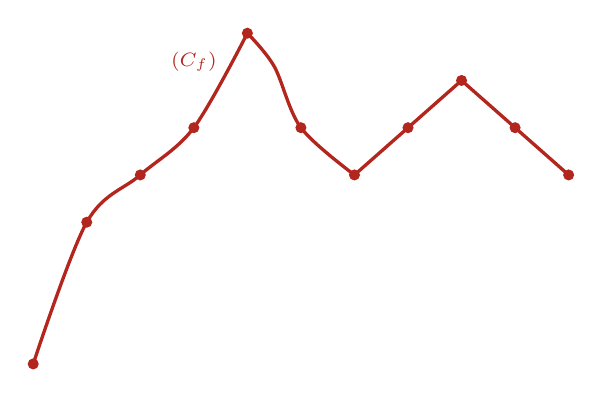
\begin{tikzpicture}[x=0.68cm,y=0.6cm,font=\scriptsize]
\Ax{-5}{5}{-4}{3}
\draw[cThm,very thick] plot[smooth,tension=0.55] coordinates{(-5,-4)(-4,-1)(-3,0)(-2,1)(-1,3)};
\draw[cThm,very thick] plot[smooth,tension=0.55] coordinates{(-1,3)(-0.5,2.3)(0,1)(1,0)};
\draw[cThm,very thick] plot[smooth,tension=0.55] coordinates{(1,0)(2,1)(3,2)};
\draw[cThm,very thick] plot[smooth,tension=0.55] coordinates{(3,2)(4,1)(5,0)};
\foreach \p in {(-5,-4),(-4,-1),(-3,0),(-2,1),(-1,3),(0,1),(1,0),(2,1),(3,2),(4,1),(5,0)} \fill[cThm] \p circle (2pt);
\node[cThm] at (-2,2.4){$(C_f)$};
\end{tikzpicture}
\end{LTR}}
\end{tamrin}
\begin{hal}
\textbf{1.} المنحنى يمتد من الفاصلة $-5$ إلى الفاصلة $5$: \ \bx{D_f=[-5;5]}.
\QQ{2} $-8\notin\Df$ ، إذن $f(-8)$ \textbf{غير موجود}. \ $f(-5)=-4$ ، $f(-3)=0$ ، $f(-1)=3$ ، $f(0)=1$ ، $f(4)=1$.
\QQ{3} سوابق $0$ (تقاطع $(C_f)$ مع محور الفواصل): \bx{-3\ ;\ 1\ ;\ 5}. \quad سوابق $1$ (تقاطع مع $y=1$): \bx{-2\ ;\ 0\ ;\ 2\ ;\ 4}.
\QQ{4} $f(x)=-1\iff x=-4$: \ $S=\{-4\}$. \quad $(C_f)$ تحت محور الفواصل من أجل $x\in[-5;-3[$: \ \bx{S=[-5;-3[}.
\QQ{5}
\begin{TAB}
\tkzTabInit[lgt=1.3,espcl=1.9]{$x$/0.7,$f(x)$/1.5}{$-5$,$-1$,$1$,$3$,$5$}
\tkzTabVar{-/$-4$,+/$3$,-/$0$,+/$2$,-/$0$}
\end{TAB}
\QQ{6} القيمة الحدية العظمى: \bx{3} عند $x=-1$. \quad القيمة الحدية الصغرى: \bx{-4} عند $x=-5$.
\end{hal}

% ------------------------------------------------- 5
\begin{tamrin}{قراءة بيانية ثم دراسة جبرية}
\RL{0.55}{%
$f$ دالة معرّفة على $\R$ ، و $(C_f)$ تمثيلها البياني (الشكل المقابل).
\begin{enumerate}
\item بقراءة بيانية:
\begin{sq}
\qa عيّن صور الأعداد $-1$ ، $0$ و $3$ بالدالة $f$.
\qb عيّن السوابق الممكنة لكل من العددين $4$ و $3$.
\qc قارن بين $f(a)$ و $f(b)$ حيث $a\in[1;2]$ و $b\in[2;3]$.
\qd عيّن إشارة $f(x)$ حسب قيم $x$.
\end{sq}
\item نفرض أن $f(x)=-x^2+2x+3$.
\begin{sq}
\qa تحقق أن: $f(x)=4-(x-1)^2$.
\qb عيّن جبرياً اتجاه تغير $f$ على كل من المجالين $]-\infty;1]$ و $[1;+\infty[$.
\qc شكّل جدول تغيرات $f$ على المجال $[-2;4]$.
\end{sq}
\end{enumerate}}{0.42}{%
\begin{LTR}\centering
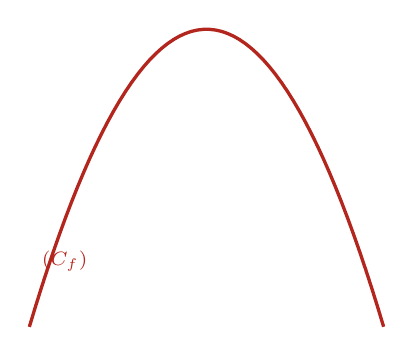
\begin{tikzpicture}[x=0.75cm,y=0.42cm,font=\scriptsize]
\Ax{-2}{4}{-5}{4}
\draw[cThm,very thick,domain=-2:4,samples=60] plot (\x,{-\x*\x+2*\x+3});
\node[cThm] at (-1.4,-3){$(C_f)$};
\end{tikzpicture}
\end{LTR}}
\end{tamrin}
\begin{hal}
\textbf{1.}
\begin{sq}
\qa $f(-1)=0$ ، $f(0)=3$ ، $f(3)=0$.
\qb سوابق $4$: العدد \bx{1} فقط (قمة المنحنى). \quad سوابق $3$: \bx{0} و \bx{2}.
\qc $f$ متناقصة على $[1;+\infty[$ ، و $a\le2\le b$ ، إذن \bx{f(a)\ge f(b)}.
\qd $f(x)>0$ من أجل $x\in\,]-1;3[$ ، $f(x)<0$ من أجل $x\in\,]-\infty;-1[\,\cup\,]3;+\infty[$ ، و $f(-1)=f(3)=0$.
\end{sq}
\QQ{2}
\begin{sq}
\qa $4-(x-1)^2=4-x^2+2x-1=-x^2+2x+3=f(x)$ \ok.
\qb ليكن $a<b$. \ على $[1;+\infty[$: $0\le a-1<b-1\Rightarrow(a-1)^2<(b-1)^2\Rightarrow-(a-1)^2>-(b-1)^2\Rightarrow f(a)>f(b)$: \textbf{متناقصة تماماً}.\par
على $]-\infty;1]$: $a-1<b-1\le0\Rightarrow(a-1)^2>(b-1)^2\Rightarrow f(a)<f(b)$: \textbf{متزايدة تماماً}.
\qc $f(-2)=4-9=-5$ ، $f(1)=4$ ، $f(4)=4-9=-5$:
\begin{TAB}
\tkzTabInit[lgt=1.3,espcl=2.4]{$x$/0.7,$f(x)$/1.4}{$-2$,$1$,$4$}
\tkzTabVar{-/$-5$,+/$4$,-/$-5$}
\end{TAB}
\end{sq}
\end{hal}

% ------------------------------------------------- 6
\begin{tamrin}{منحنى ومستقيم: حل بياني وجبري}
\RL{0.55}{%
$f$ الدالة المعرّفة على $[-2;4]$ بتمثيلها البياني $(C_f)$ ، و $g$ الدالة المعرّفة على $[-1;4]$ بـ: $g(x)=x-3$ ، و $(C_g)$ تمثيلها البياني (الشكل).
\begin{enumerate}
\item عيّن $\Df$ ، ثم صور العددين $-2$ و $0$ بالدالة $f$.
\item عيّن السوابق الممكنة لكل من العددين $-3$ و $0$ بالدالة $f$.
\item هل تقبل $f$ قيمة حدية صغرى؟ عيّنها إن وجدت.
\item عيّن اتجاه تغير $f$ ثم شكّل جدول تغيراتها.
\item ادرس شفعية الدالة $g$.
\item حل بيانياً في $[-1;4]$ المعادلة $f(x)=g(x)$ والمتراجحة $f(x)<g(x)$.
\item نقبل أن $f(x)=x^2-2x-3$. \ تحقق جبرياً من نتائج السؤال 6.
\end{enumerate}}{0.42}{%
\begin{LTR}\centering
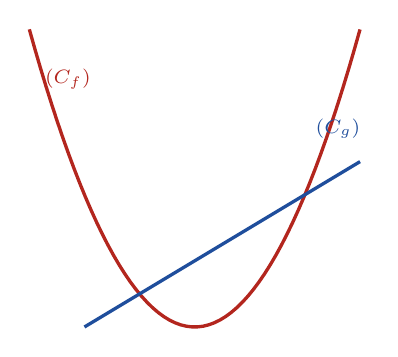
\begin{tikzpicture}[x=0.7cm,y=0.42cm,font=\scriptsize]
\Ax{-2}{4}{-5}{5}
\draw[cThm,very thick,domain=-2:4,samples=60] plot (\x,{\x*\x-2*\x-3});
\draw[cDef,very thick] (-1,-4)--(4,1);
\node[cThm] at (-1.3,3.5){$(C_f)$}; \node[cDef] at (3.6,2){$(C_g)$};
\end{tikzpicture}
\end{LTR}}
\end{tamrin}
\begin{hal}
\textbf{1.} \bx{D_f=[-2;4]} ، \ $f(-2)=5$ ، $f(0)=-3$.
\QQ{2} سوابق $-3$: \bx{0} و \bx{2}. \quad سوابق $0$: \bx{-1} و \bx{3}.
\QQ{3} نعم: القيمة الحدية الصغرى \bx{-4} عند $x=1$.
\QQ{4} $f$ متناقصة تماماً على $[-2;1]$ ومتزايدة تماماً على $[1;4]$:
\begin{TAB}
\tkzTabInit[lgt=1.3,espcl=2.4]{$x$/0.7,$f(x)$/1.4}{$-2$,$1$,$4$}
\tkzTabVar{+/$5$,-/$-4$,+/$5$}
\end{TAB}
\QQ{5} $D_g=[-1;4]$ \textbf{ليست متناظرة} بالنسبة إلى $0$ ($4\in D_g$ لكن $-4\notin D_g$): \ $g$ \textbf{لا زوجية ولا فردية}.
\QQ{6} $(C_f)$ و $(C_g)$ يتقاطعان في $(0;-3)$ و $(3;0)$: \ حلول $f(x)=g(x)$: \bx{S=\{0;3\}}.\par
$(C_f)$ تحت $(C_g)$ بين الفاصلتين $0$ و $3$: \ حلول $f(x)<g(x)$: \bx{S=\,]0;3[}.
\QQ{7} $f(x)=g(x)\iff x^2-2x-3=x-3\iff x^2-3x=0\iff x(x-3)=0$: \ $x=0$ أو $x=3$ \ok.\par
$f(x)-g(x)=x(x-3)<0$ بين الجذرين $0$ و $3$ \ok.
\end{hal}

% ------------------------------------------------- 7
\begin{tamrin}{إشارة دالة ومقارنة صور}
\RL{0.55}{%
$(C_f)$ هو التمثيل البياني لدالة $f$ (الشكل المقابل).
\begin{enumerate}
\item عيّن $\Df$ ، ثم صور الأعداد $-1$ ، $2$ و $5$ بالدالة $f$.
\item عيّن السوابق الممكنة للعدد $0$.
\item عيّن القيم الحدية للدالة $f$.
\item عيّن اتجاه تغير $f$ ثم شكّل جدول تغيراتها.
\item قارن بين $f(-2)$ و $f(-1{,}5)$ دون حساب.
\item عيّن إشارة الدالة $f$ ، ثم استنتج حلول المتراجحة $f(x)\ge0$.
\end{enumerate}}{0.42}{%
\begin{LTR}\centering
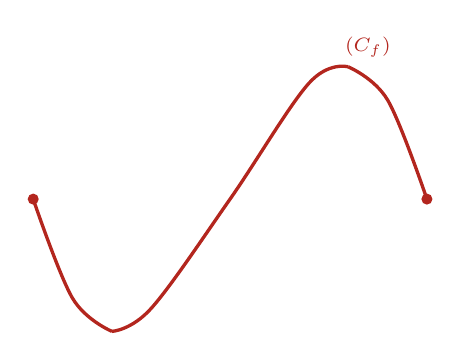
\begin{tikzpicture}[x=0.5cm,y=0.42cm,font=\scriptsize]
\Ax{-3}{7}{-4}{4}
\draw[cThm,very thick] plot[smooth,tension=0.6] coordinates{(-3,0)(-2,-3)(-1,-4)};
\draw[cThm,very thick] plot[smooth,tension=0.6] coordinates{(-1,-4)(0,-3.3)(2,0)(4,3.5)(5,4)};
\draw[cThm,very thick] plot[smooth,tension=0.6] coordinates{(5,4)(6,3)(7,0)};
\fill[cThm] (-3,0) circle (2pt) (7,0) circle (2pt);
\node[cThm] at (5.5,4.6){$(C_f)$};
\end{tikzpicture}
\end{LTR}}
\end{tamrin}
\begin{hal}
\textbf{1.} \bx{D_f=[-3;7]} ، \ $f(-1)=-4$ ، $f(2)=0$ ، $f(5)=4$.
\QQ{2} سوابق $0$: \bx{-3\ ;\ 2\ ;\ 7}.
\QQ{3} القيمة الحدية العظمى \bx{4} عند $x=5$ ، والصغرى \bx{-4} عند $x=-1$.
\QQ{4}
\begin{TAB}
\tkzTabInit[lgt=1.3,espcl=2.2]{$x$/0.7,$f(x)$/1.4}{$-3$,$-1$,$5$,$7$}
\tkzTabVar{+/$0$,-/$-4$,+/$4$,-/$0$}
\end{TAB}
\QQ{5} $-2$ و $-1{,}5$ ينتميان إلى $[-3;-1]$ حيث $f$ متناقصة تماماً ، و $-2<-1{,}5$ ، إذن \bx{f(-2)>f(-1{,}5)}.
\QQ{6} $f(x)\le0$ على $[-3;2]$ ، و $f(x)\ge0$ على $[2;7]$ ، مع $f(-3)=f(2)=f(7)=0$.\par
حلول $f(x)\ge0$: \bx{S=\{-3\}\cup[2;7]}.
\end{hal}

% ------------------------------------------------- 8
\begin{tamrin}{دالة معرّفة بجدول تغيراتها}
$f$ دالة معرّفة بجدول تغيراتها التالي:
\begin{TAB}
\tkzTabInit[lgt=1.3,espcl=1.6]{$x$/0.7,$f(x)$/1.6}{$-4$,$-1$,$0$,$1$,$3$,$5$}
\tkzTabVar{+/$1{,}5$,R/,-/$-2$,R/,+/$2$,-/$1$}
\tkzTabIma{1}{3}{2}{$0$}
\tkzTabIma{3}{5}{4}{$0$}
\end{TAB}
\begin{enumerate}
\item عيّن $\Df$. \ هل الدالة $f$ زوجية؟
\item عيّن القيم الحدية للدالة $f$.
\item حل في $\Df$ المعادلة $f(x)=0$ ، ثم عيّن إشارة $f(x)$.
\item قارن دون حساب ومع التعليل بين: $f(-3)$ و $f(-2)$ ، ثم بين $f\Big(\dfrac12\Big)$ و $f(2)$.
\item ارسم منحنياً ممكناً للدالة $f$.
\end{enumerate}
\end{tamrin}
\begin{hal}
\textbf{1.} \bx{D_f=[-4;5]}. \ $\Df$ ليست متناظرة ($5\in\Df$ و $-5\notin\Df$) ، إذن $f$ \textbf{ليست زوجية}.
\QQ{2} القيمة الحدية العظمى \bx{2} عند $x=3$ ، والصغرى \bx{-2} عند $x=0$.
\QQ{3} من الجدول: $f(-1)=0$ و $f(1)=0$ ، ولا تنعدم في مكان آخر (القيم على $[3;5]$ بين $1$ و $2$): \ \bx{S=\{-1;1\}}.
\RL{0.52}{%
\begin{TAB}
\tkzTabInit[lgt=1.3,espcl=1.7]{$x$/0.7,$f(x)$/0.7}{$-4$,$-1$,$1$,$5$}
\tkzTabLine{,+,z,-,z,+,}
\end{TAB}}{0.45}{%
\QQ{4} $-3<-2$ في $[-4;0]$ حيث $f$ متناقصة: \bx{f(-3)>f(-2)}.\par
$\dfrac12<2$ في $[0;3]$ حيث $f$ متزايدة: \bx{f\Big(\dfrac12\Big)<f(2)}.}
\RL{0.48}{%
\QQ{5} منحنٍ ممكن (الشكل) ، يمر بالنقط:\par
$(-4;1{,}5)$ ، $(-1;0)$ ، $(0;-2)$ ، $(1;0)$ ، $(3;2)$ و $(5;1)$ ، ويحترم اتجاه التغير.}{0.49}{%
\begin{LTR}\centering
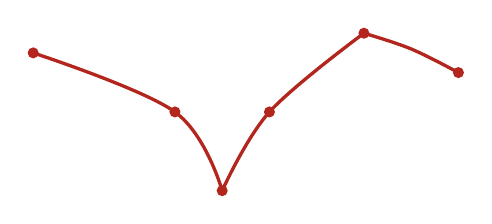
\begin{tikzpicture}[x=0.6cm,y=0.5cm,font=\scriptsize]
\Ax{-4}{5}{-2}{2}
\draw[cThm,very thick] plot[smooth,tension=0.6] coordinates{(-4,1.5)(-1,0)(0,-2)};
\draw[cThm,very thick] plot[smooth,tension=0.6] coordinates{(0,-2)(1,0)(3,2)};
\draw[cThm,very thick] plot[smooth,tension=0.6] coordinates{(3,2)(4,1.6)(5,1)};
\foreach \p in {(-4,1.5),(-1,0),(0,-2),(1,0),(3,2),(5,1)} \fill[cThm] \p circle (2pt);
\end{tikzpicture}
\end{LTR}}
\end{hal}

% =====================================================================
\section{الشفعية واتجاه التغير والقيم الحدية}
% ------------------------------------------------- 9
\begin{tamrin}{دراسة الشفعية}
\begin{enumerate}
\item ادرس شفعية كل دالة مما يلي:
\begin{sq}
\qa $f_1(x)=3x^2-5$
\qb $f_2(x)=x^3-3x$
\qc $f_3(x)=\dfrac{x^2+1}{x}$
\qd $f_4(x)=|x|+x^2$
\qe $f_5(x)=\sqrt{x+2}$
\end{sq}
\item $h$ الدالة المعرّفة على $[-2;2]$ بـ: $h(x)=x^3-3x$. \ احسب $h(2)$ ثم استنتج $h(-2)$ دون حساب ، وحل المعادلة $h(x)=x$.
\item $f$ دالة \textbf{فردية} على $\R$ حيث $f\big(\sqrt2\big)=9-6\sqrt2$. \ عيّن $f\big(-\sqrt2\big)$ و $f(0)$.
\end{enumerate}
\end{tamrin}
\begin{hal}
\textbf{1.}
\begin{sq}
\qa $D=\R$ متناظرة ، $f_1(-x)=3(-x)^2-5=3x^2-5=f_1(x)$: \ \textbf{زوجية}.
\qb $D=\R$ ، $f_2(-x)=(-x)^3-3(-x)=-x^3+3x=-\big(x^3-3x\big)=-f_2(x)$: \ \textbf{فردية}.
\qc $D=\R^*$ متناظرة ، $f_3(-x)=\dfrac{x^2+1}{-x}=-f_3(x)$: \ \textbf{فردية}.
\qd $D=\R$ ، $f_4(-x)=|-x|+(-x)^2=|x|+x^2=f_4(x)$: \ \textbf{زوجية}.
\qe $D=[-2;+\infty[$ ليست متناظرة ($3\in D$ و $-3\notin D$): \ \textbf{لا زوجية ولا فردية}.
\end{sq}
\QQ{2} $h(2)=8-6=\bx{2}$. \ $[-2;2]$ متناظر و $h$ فردية (كما في 1(ب)) ، إذن $h(-2)=-h(2)=\bx{-2}$.\par
$h(x)=x\iff x^3-4x=0\iff x(x-2)(x+2)=0$: \ \bx{S=\{-2;0;2\}}.
\QQ{3} $f\big(-\sqrt2\big)=-f\big(\sqrt2\big)=\bx{-9+6\sqrt2}$. \quad و $f(-0)=-f(0)$ ، أي $f(0)=-f(0)$ ، ومنه \bx{f(0)=0}.
\end{hal}

% ------------------------------------------------- 10
\begin{tamrin}{الشكل النموذجي وقيمة حدية}
$f$ الدالة المعرّفة على $\R$ بـ: $f(x)=4x^2-12x+5$.
\begin{enumerate}
\item تحقق أنه من أجل كل $x$ من $\R$: \ $f(x)=(2x-3)^2-4$.
\item احسب كلاً من $f(-1)$ و $f(0)$ ، ثم حل في $\R$ المعادلة $f(x)=0$.
\item ادرس اتجاه تغير $f$ على كل من المجالين $\Big]-\infty;\dfrac32\Big]$ و $\Big[\dfrac32;+\infty\Big[$ ، ثم شكّل جدول تغيراتها.
\item استنتج أنه من أجل كل $x$ من $\R$: \ $f(x)-f\Big(\dfrac32\Big)\ge0$. \ ماذا تمثل $f\Big(\dfrac32\Big)$ بالنسبة لـ $f$؟
\end{enumerate}
\end{tamrin}
\begin{hal}
\textbf{1.} $(2x-3)^2-4=4x^2-12x+9-4=4x^2-12x+5=f(x)$ \ok.
\QQ{2} $f(-1)=4+12+5=\bx{21}$ ، $f(0)=\bx{5}$.\par
$f(x)=0\iff(2x-3)^2=4\iff2x-3=2$ أو $2x-3=-2\iff x=\dfrac52$ أو $x=\dfrac12$: \ \bx{S=\Big\{\dfrac12;\dfrac52\Big\}}.
\QQ{3} ليكن $a<b$. \ على $\Big[\dfrac32;+\infty\Big[$: $0\le2a-3<2b-3\Rightarrow(2a-3)^2<(2b-3)^2\Rightarrow f(a)<f(b)$: \textbf{متزايدة تماماً}.\par
على $\Big]-\infty;\dfrac32\Big]$: $2a-3<2b-3\le0\Rightarrow(2a-3)^2>(2b-3)^2\Rightarrow f(a)>f(b)$: \textbf{متناقصة تماماً}.
\begin{TAB}
\tkzTabInit[lgt=1.3,espcl=2.4]{$x$/0.7,$f(x)$/1.4}{$-\infty$,$\frac32$,$+\infty$}
\tkzTabVar{+/,-/$-4$,+/}
\end{TAB}
\QQ{4} $f\Big(\dfrac32\Big)=0-4=-4$ ، و $f(x)-f\Big(\dfrac32\Big)=(2x-3)^2\ge0$.\par
إذن $f(x)\ge f\Big(\dfrac32\Big)$ لكل $x$: \ $f\Big(\dfrac32\Big)=-4$ هي \textbf{القيمة الحدية الصغرى} لـ $f$.
\end{hal}

% ------------------------------------------------- 11
\begin{tamrin}{دالة مقصورة على مجال}
$f$ الدالة المعرّفة على المجال $[-3;1]$ بـ: $f(x)=3(x+1)^2-7$.
\begin{enumerate}
\item احسب كلاً من $f(-3)$ ، $f(1)$ و $f(0)$.
\item عيّن السوابق الممكنة للعدد $-7$ بالدالة $f$.
\item ادرس اتجاه تغير $f$ على كل من المجالين $[-3;-1]$ و $[-1;1]$ ، ثم شكّل جدول تغيراتها.
\item عيّن قيمة حدية للدالة $f$.
\item قارن دون حساب ومع التعليل بين $f(0{,}5)$ و $f(0{,}75)$.
\end{enumerate}
\end{tamrin}
\begin{hal}
\textbf{1.} $f(-3)=3\times4-7=\bx{5}$ ، $f(1)=3\times4-7=\bx{5}$ ، $f(0)=3-7=\bx{-4}$.
\QQ{2} $f(x)=-7\iff3(x+1)^2=0\iff x=-1\in[-3;1]$: \ سابقة وحيدة \bx{-1}.
\QQ{3} ليكن $a<b$. \ على $[-1;1]$: $0\le a+1<b+1\Rightarrow(a+1)^2<(b+1)^2\Rightarrow3(a+1)^2-7<3(b+1)^2-7$: \textbf{متزايدة تماماً}.\par
على $[-3;-1]$: $a+1<b+1\le0\Rightarrow(a+1)^2>(b+1)^2\Rightarrow f(a)>f(b)$: \textbf{متناقصة تماماً}.
\begin{TAB}
\tkzTabInit[lgt=1.3,espcl=2.4]{$x$/0.7,$f(x)$/1.4}{$-3$,$-1$,$1$}
\tkzTabVar{+/$5$,-/$-7$,+/$5$}
\end{TAB}
\QQ{4} $(x+1)^2\ge0$ ، إذن $f(x)\ge-7=f(-1)$: \ القيمة الحدية الصغرى \bx{-7} عند $x=-1$ (والعظمى $5$ عند $-3$ و $1$).
\QQ{5} $0{,}5<0{,}75$ في $[-1;1]$ حيث $f$ متزايدة تماماً: \ \bx{f(0{,}5)<f(0{,}75)} \ (تحقق: $-0{,}25<2{,}1875$ \ok).
\end{hal}

% ------------------------------------------------- 12
\begin{tamrin}{دالة كسرية: اتجاه التغير بالفرق}
$f$ الدالة المعرّفة على $\R-\Big\{-\dfrac12\Big\}$ بـ: $f(x)=\dfrac{x+3}{2x+1}$.
\begin{enumerate}
\item احسب صور الأعداد $-1$ ، $0$ و $2$ بالدالة $f$.
\item عيّن السوابق الممكنة لكل من العددين $-2$ و $\dfrac12$.
\item أثبت أنه من أجل كل $x_1$ و $x_2$ من $\R-\Big\{-\dfrac12\Big\}$: \ $f(x_1)-f(x_2)=\dfrac{5(x_2-x_1)}{(2x_1+1)(2x_2+1)}$.
\item استنتج اتجاه تغير $f$ على كل من المجالين $\Big]-\infty;-\dfrac12\Big[$ و $\Big]-\dfrac12;+\infty\Big[$ ، ثم شكّل جدول تغيراتها.
\item هل الدالة $f$ فردية؟ علّل.
\end{enumerate}
\end{tamrin}
\begin{hal}
\textbf{1.} $f(-1)=\dfrac{2}{-1}=\bx{-2}$ ، $f(0)=\bx{3}$ ، $f(2)=\dfrac55=\bx{1}$.
\QQ{2} $f(x)=-2\iff x+3=-4x-2\iff5x=-5\iff x=-1$: \ سابقة وحيدة \bx{-1}.\par
$f(x)=\dfrac12\iff2x+6=2x+1\iff6=1$: مستحيل ، إذن $\dfrac12$ \textbf{ليس له سابقة}.
\QQ{3} بتوحيد المقامات:
\begin{align*}
f(x_1)-f(x_2)&=\frac{(x_1+3)(2x_2+1)-(x_2+3)(2x_1+1)}{(2x_1+1)(2x_2+1)}\\
&=\frac{2x_1x_2+x_1+6x_2+3-2x_1x_2-x_2-6x_1-3}{(2x_1+1)(2x_2+1)}=\frac{5(x_2-x_1)}{(2x_1+1)(2x_2+1)}.
\end{align*}
\QQ{4} ليكن $x_1<x_2$ ، إذن $x_2-x_1>0$.
\begin{itemize}
\item على $\Big]-\dfrac12;+\infty\Big[$: $2x_1+1>0$ و $2x_2+1>0$ ، فالمقام موجب و $f(x_1)-f(x_2)>0$: \textbf{متناقصة تماماً}.
\item على $\Big]-\infty;-\dfrac12\Big[$: العاملان سالبان وجداؤهما موجب ، و $f(x_1)-f(x_2)>0$: \textbf{متناقصة تماماً}.
\end{itemize}
\begin{TAB}
\tkzTabInit[lgt=1.3,espcl=2.6]{$x$/0.7,$f(x)$/1.4}{$-\infty$,$-\frac12$,$+\infty$}
\tkzTabVar{+/,-D+/,-/}
\end{TAB}
\QQ{5} $\Df$ ليست متناظرة ($\dfrac12\in\Df$ و $-\dfrac12\notin\Df$) ، إذن $f$ \textbf{ليست فردية}.
\end{hal}

% ------------------------------------------------- 13
\begin{tamrin}{مقارنة دالتين بجدول الإشارة}
\begin{enumerate}
\item $f(x)=x^2+ax+b$ دالة معرّفة على $\R$. \ نعلم أن $(C_f)$ يقطع محور التراتيب في النقطة ذات الترتيب $1$ ومحور الفواصل في النقطة ذات الفاصلة $-1$. \ عيّن $a$ و $b$ ، ثم بيّن أن $f(x)=(x+1)^2$.
\item هل الدالة $f$ زوجية؟ ادرس اتجاه تغيرها وشكّل جدول تغيراتها.
\item $g$ الدالة المعرّفة بـ: $g(x)=\dfrac{3x+3}{x-1}$.
\begin{sq}
\qa عيّن $D_g$ ، ثم بيّن أنه من أجل كل $x$ من $D_g$: $g(x)=3+\dfrac{6}{x-1}$.
\qb حل في $\R$ المعادلة $g(x)=0$. ماذا تستنتج؟
\qc بيّن أنه من أجل كل $x\ne1$: \ $f(x)-g(x)=\dfrac{(x+1)(x-2)(x+2)}{x-1}$.
\qd حل المعادلة $f(x)-g(x)=0$ ، واستنتج فواصل نقط تقاطع $(C_f)$ و $(C_g)$.
\qe ادرس إشارة $f(x)-g(x)$ ، ثم استنتج حلول المتراجحة $f(x)>g(x)$.
\end{sq}
\end{enumerate}
\end{tamrin}
\begin{hal}
\textbf{1.} $f(0)=1$ ، أي \bx{b=1}. \quad $f(-1)=0$ ، أي $1-a+1=0$ ، \bx{a=2}. \quad إذن $f(x)=x^2+2x+1=(x+1)^2$.
\QQ{2} $f(-1)=0$ و $f(1)=4$: \ $f(-1)\ne f(1)$ ، إذن $f$ \textbf{ليست زوجية}.\par
ليكن $a<b$: على $[-1;+\infty[$: $0\le a+1<b+1\Rightarrow f(a)<f(b)$ (متزايدة) ؛ على $]-\infty;-1]$: $a+1<b+1\le0\Rightarrow f(a)>f(b)$ (متناقصة).
\begin{TAB}
\tkzTabInit[lgt=1.3,espcl=2.4]{$x$/0.7,$f(x)$/1.4}{$-\infty$,$-1$,$+\infty$}
\tkzTabVar{+/,-/$0$,+/}
\end{TAB}
\QQ{3}
\begin{sq}
\qa $x-1\ne0$: \ \bx{D_g=\R-\{1\}}. \quad $3+\dfrac{6}{x-1}=\dfrac{3(x-1)+6}{x-1}=\dfrac{3x+3}{x-1}=g(x)$ \ok.
\qb $g(x)=0\iff3x+3=0$ و $x\ne1\iff x=-1$: \ $S=\{-1\}$. \ نستنتج أن $(C_g)$ يقطع محور الفواصل في $(-1;0)$ ، وهي نقطة من $(C_f)$ أيضاً لأن $f(-1)=0$.
\qc $f(x)-g(x)=(x+1)^2-\dfrac{3(x+1)}{x-1}=\dfrac{(x+1)\big[(x+1)(x-1)-3\big]}{x-1}=\dfrac{(x+1)(x^2-4)}{x-1}=\dfrac{(x+1)(x-2)(x+2)}{x-1}$ \ok.
\qd $f(x)-g(x)=0\iff x=-1$ أو $x=2$ أو $x=-2$: \ $(C_f)$ و $(C_g)$ يتقاطعان في النقط ذات الفواصل \bx{-2\ ;\ -1\ ;\ 2}.
\qe جدول الإشارة:
\begin{TAB}
\tkzTabInit[lgt=2.2,espcl=1.5]{$x$/0.7,$x+2$/0.6,$x+1$/0.6,$x-1$/0.6,$x-2$/0.6,$f(x)-g(x)$/0.7}{$-\infty$,$-2$,$-1$,$1$,$2$,$+\infty$}
\tkzTabLine{,-,z,+,t,+,t,+,t,+,}
\tkzTabLine{,-,t,-,z,+,t,+,t,+,}
\tkzTabLine{,-,t,-,t,-,z,+,t,+,}
\tkzTabLine{,-,t,-,t,-,t,-,z,+,}
\tkzTabLine{,+,z,-,z,+,d,-,z,+,}
\end{TAB}
حلول $f(x)>g(x)$: \ \bx{S=\,]-\infty;-2[\,\cup\,]-1;1[\,\cup\,]2;+\infty[}.
\end{sq}
\end{hal}

% ------------------------------------------------- 14
\begin{tamrin}{دالة من الدرجة الثالثة}
\RL{0.58}{%
$f$ الدالة المعرّفة على $\R$ بـ: $f(x)=x^3-3x^2+4$ ، و $(C_f)$ تمثيلها البياني (الشكل).
\begin{enumerate}
\item بقراءة بيانية: عيّن صور الأعداد $-1$ ، $0$ ، $2$ و $3$ ، ثم سوابق العدد $4$.
\item
\begin{sq}
\qa تحقق أنه من أجل كل $x$ من $\R$: \ $f(x)=(x+1)(x-2)^2$.
\qb حل جبرياً المعادلتين: $f(x)=0$ و $f(x)=4$.
\end{sq}
\item في المجال $[-1;1]$:
\begin{sq}
\qa احسب الفرق $f(x)-f(0)$.
\qb استنتج مقارنة بين $f(x)$ و $f(0)$. ماذا يمثل العدد $f(0)$؟
\end{sq}
\end{enumerate}}{0.39}{%
\begin{LTR}\centering
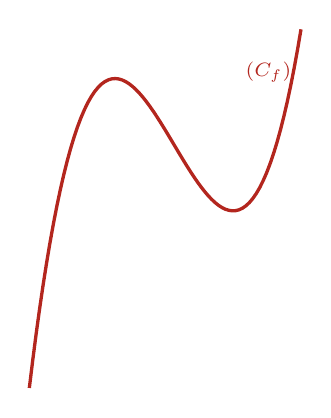
\begin{tikzpicture}[x=0.75cm,y=0.42cm,font=\scriptsize]
\Ax{-2}{3}{-4}{5}
\draw[cThm,very thick,domain=-1.45:3.15,samples=80] plot (\x,{\x*\x*\x-3*\x*\x+4});
\node[cThm] at (2.6,4.2){$(C_f)$};
\end{tikzpicture}
\end{LTR}}
\end{tamrin}
\begin{hal}
\textbf{1.} $f(-1)=0$ ، $f(0)=4$ ، $f(2)=0$ ، $f(3)=4$. \quad سوابق $4$: \bx{0} و \bx{3}.
\QQ{2}
\begin{sq}
\qa $(x+1)(x-2)^2=(x+1)\big(x^2-4x+4\big)=x^3-4x^2+4x+x^2-4x+4=x^3-3x^2+4$ \ok.
\qb $f(x)=0\iff x=-1$ أو $x=2$: \ \bx{S=\{-1;2\}}. \quad $f(x)=4\iff x^3-3x^2=0\iff x^2(x-3)=0$: \ \bx{S=\{0;3\}}.
\end{sq}
\QQ{3}
\begin{sq}
\qa $f(x)-f(0)=x^3-3x^2=\bx{x^2(x-3)}$.
\qb على $[-1;1]$: $x^2\ge0$ و $x-3<0$ ، إذن $f(x)-f(0)\le0$ ، أي $f(x)\le f(0)$.\par
$f(0)=4$ هي \textbf{القيمة الحدية العظمى} لـ $f$ على المجال $[-1;1]$.
\end{sq}
\end{hal}

% =====================================================================
\section{وضعيات إدماجية (تمارين نموذجية)}
% ------------------------------------------------- 15
\begin{tamrin}{أكبر مستطيل داخل مثلث}
\RL{0.58}{%
$ABC$ مثلث متساوي الساقين رأسه الأساسي $A$ حيث $AB=AC=5\,cm$ و $BC=8\,cm$ ، و $H$ المسقط العمودي لـ $A$ على $(BC)$.\par
نضع $BM=NC=x$ ، والرباعي $PQMN$ مستطيل ($M$ و $N$ على $[BC]$ ، $Q\in[AB]$ ، $P\in[AC]$).
\begin{enumerate}
\item حدّد المجال الذي ينتمي إليه $x$.
\item احسب الطول $AH$ ، ثم بيّن أن $MQ=\dfrac34x$ (استعمل مبرهنة طالس).
\item نسمي $S$ مساحة المستطيل $PQMN$. \ بيّن أن $S=f(x)$ حيث: $f(x)=-\dfrac32x^2+6x$.
\item احسب $f(0)$ ، $f(2)$ و $f(4)$.
\item بيّن أنه يمكن كتابة $f(x)=-\dfrac32\big[(x+a)^2+b\big]$ حيث $a$ و $b$ عددان حقيقيان يطلب تعيينهما.
\item ادرس اتجاه تغير $f$ على المجالين $[0;2]$ و $[2;4]$ ، ثم شكّل جدول تغيراتها.
\item عيّن قيمة $x$ حتى تكون مساحة المستطيل أكبر ما يمكن.
\end{enumerate}}{0.39}{%
\begin{LTR}\centering
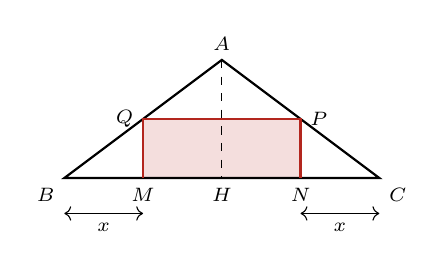
\begin{tikzpicture}[scale=0.5,font=\scriptsize]
\coordinate (B) at (0,0); \coordinate (C) at (8,0); \coordinate (A) at (4,3); \coordinate (H) at (4,0);
\fill[cThm!15] (2,0) rectangle (6,1.5);
\draw[thick] (B)--(A)--(C)--cycle; \draw[dashed] (A)--(H);
\draw[cThm,thick] (2,0)--(2,1.5)--(6,1.5)--(6,0);
\node[below left] at (B){$B$}; \node[below right] at (C){$C$}; \node[above] at (A){$A$}; \node[below] at (H){$H$};
\node[below] at (2,0){$M$}; \node[below] at (6,0){$N$}; \node[left] at (2,1.5){$Q$}; \node[right] at (6,1.5){$P$};
\draw[<->] (0,-0.9)--(2,-0.9) node[midway,below]{$x$}; \draw[<->] (6,-0.9)--(8,-0.9) node[midway,below]{$x$};
\end{tikzpicture}
\end{LTR}}
\end{tamrin}
\begin{hal}
\textbf{1.} $M$ بين $B$ و $H$ ، و $BH=\dfrac{BC}2=4$: \ \bx{x\in[0;4]}.
\QQ{2} في المثلث $ABH$ القائم في $H$ (فيثاغورس): $AH^2=AB^2-BH^2=25-16=9$ ، \bx{AH=3\,cm}.\par
$(QM)\parallel(AH)$ (كلاهما عمودي على $(BC)$) ، وحسب طالس في المثلث $ABH$: $\dfrac{BM}{BH}=\dfrac{QM}{AH}$ ، أي $QM=\dfrac{x\times3}{4}=\bx{\dfrac34x}$.
\QQ{3} $MN=BC-2x=8-2x$ ، و $S=MQ\times MN=\dfrac34x(8-2x)=6x-\dfrac32x^2=f(x)$ \ok.
\QQ{4} $f(0)=\bx{0}$ ، $f(2)=-6+12=\bx{6}$ ، $f(4)=-24+24=\bx{0}$.
\QQ{5} $f(x)=-\dfrac32\big[x^2-4x\big]=-\dfrac32\big[(x-2)^2-4\big]$: \ \bx{a=-2} و \bx{b=-4}.
\QQ{6} $f(x)=-\dfrac32(x-2)^2+6$. \ ليكن $a'<b'$:\par
على $[2;4]$: $0\le a'-2<b'-2\Rightarrow(a'-2)^2<(b'-2)^2\Rightarrow f(a')>f(b')$: \textbf{متناقصة تماماً}.\par
على $[0;2]$: $a'-2<b'-2\le0\Rightarrow(a'-2)^2>(b'-2)^2\Rightarrow f(a')<f(b')$: \textbf{متزايدة تماماً}.
\begin{TAB}
\tkzTabInit[lgt=1.3,espcl=2.4]{$x$/0.7,$f(x)$/1.4}{$0$,$2$,$4$}
\tkzTabVar{-/$0$,+/$6$,-/$0$}
\end{TAB}
\QQ{7} القيمة الحدية العظمى \bx{6\,cm^2} عند \bx{x=2} ، أي $M$ منتصف $[BH]$ ، والمستطيل بعداه $MN=4$ و $MQ=1{,}5$.
\end{hal}

% ------------------------------------------------- 16
\begin{tamrin}{مستطيل داخل مثلث قائم}
$ABC$ مثلث قائم في $A$ ومتساوي الساقين حيث $AB=AC=6\,cm$. \ $M$ نقطة متغيرة من $[AB]$ ، و $P$ نقطة من $[AC]$ حيث $AM=CP=x$ مع $x\in[0;6]$ ، و $N$ نقطة من $[BC]$ بحيث يكون $AMNP$ مستطيلاً.
\begin{enumerate}
\item نضع $f(x)$ مساحة المستطيل $AMNP$.
\begin{sq}
\qa عيّن مساحة المستطيل $AMNP$ بدلالة $x$.
\qb تحقق أن: $f(x)=-(x-3)^2+9$.
\end{sq}
\item عيّن قيمة $x$ حتى تكون مساحة $AMNP$ تساوي نصف مساحة المثلث $ABC$.
\item عيّن قيم $x$ حتى تكون مساحة $AMNP$ أصغر من أو تساوي $5\,cm^2$.
\item إذا علمت أن $f$ متزايدة تماماً على $[0;3]$ ومتناقصة تماماً على $[3;6]$ ، عيّن موضع $M$ حتى تكون مساحة $AMNP$ أكبر ما يمكن ، وما قيمتها؟
\end{enumerate}
\end{tamrin}
\begin{hal}
\textbf{1.}
\begin{sq}
\qa $AP=AC-CP=6-x$ ، و $AM=x$: \ $f(x)=AM\times AP=\bx{x(6-x)=6x-x^2}$.
\qb $-(x-3)^2+9=-x^2+6x-9+9=-x^2+6x=f(x)$ \ok.
\end{sq}
\QQ{2} $S_{ABC}=\dfrac{6\times6}{2}=18$ ، نصفها $9$: \ $f(x)=9\iff(x-3)^2=0\iff\bx{x=3}$.
\QQ{3} $f(x)\le5\iff-(x-3)^2+9\le5\iff(x-3)^2\ge4\iff x-3\le-2$ أو $x-3\ge2\iff x\le1$ أو $x\ge5$.\par
مع $x\in[0;6]$: \ \bx{x\in[0;1]\cup[5;6]}.
\QQ{4} حسب اتجاه التغير ، أكبر قيمة هي $f(3)=\bx{9\,cm^2}$ عند $x=3$: $M$ \textbf{منتصف} $[AB]$ ، والمستطيل عندئذ مربع ضلعه $3\,cm$.
\end{hal}

% ------------------------------------------------- 17
\begin{tamrin}{مساحة مربع متغير}
$[AB]$ قطعة مستقيمة حيث $AB=5\,cm$ ، و $M$ نقطة تتحرك على $[AB]$ حيث $AM=x$. \ على نصف المستقيم العمودي على $(AB)$ في $B$ نضع النقطة $N$ حيث $BN=2AM$. \ نعتبر $f(x)$ مساحة المربع $MNEF$ (ضلعه $[MN]$).
\begin{enumerate}
\item عيّن المجال الذي ينتمي إليه $x$.
\item احسب الأطوال $MB$ و $BN$ بدلالة $x$ ، ثم بيّن أن: $f(x)=4x^2+(5-x)^2$.
\item عيّن قيمة $f(x)$ من أجل $x=3$.
\item تحقق أن: $f(x)=5x^2-10x+25$ و $f(x)=5(x-1)^2+20$.
\item حل المعادلة $f(x)=65$ ، ثم استنتج قيمة $x$ التي تكون من أجلها مساحة المربع $65\,cm^2$.
\item عيّن أصغر مساحة ممكنة للمربع $MNEF$ وقيمة $x$ الموافقة.
\end{enumerate}
\end{tamrin}
\begin{hal}
\textbf{1.} $M\in[AB]$: \ \bx{x\in[0;5]}.
\QQ{2} $MB=\bx{5-x}$ و $BN=\bx{2x}$. \ المثلث $MBN$ قائم في $B$ (فيثاغورس): $MN^2=MB^2+BN^2=(5-x)^2+4x^2$ ، و $f(x)=MN^2$ \ok.
\QQ{3} $f(3)=4\times9+4=\bx{40\,cm^2}$.
\QQ{4} $4x^2+25-10x+x^2=5x^2-10x+25$ \ok ، و $5(x-1)^2+20=5x^2-10x+5+20=5x^2-10x+25$ \ok.
\QQ{5} $f(x)=65\iff5(x-1)^2=45\iff(x-1)^2=9\iff x=4$ أو $x=-2$.\par
$-2\notin[0;5]$ ، إذن \bx{x=4} \ (تحقق: $f(4)=64+1=65$ \ok).
\QQ{6} $(x-1)^2\ge0$ ، إذن $f(x)\ge20=f(1)$: \ أصغر مساحة \bx{20\,cm^2} من أجل \bx{x=1}.
\end{hal}

% =====================================================================
\section{صحيح أم خطأ ، اختيار من متعدد}
% ------------------------------------------------- 18
\begin{tamrin}{صحيح أم خطأ انطلاقاً من جدول التغيرات}
$f$ دالة معرّفة على $D=[-1;5]$ وجدول تغيراتها كما يلي:
\begin{TAB}
\tkzTabInit[lgt=1.3,espcl=1.8]{$x$/0.7,$f(x)$/1.6}{$-1$,$0$,$2$,$4$,$5$}
\tkzTabVar{+/$2$,R/,-/$-1$,+/$3$,-/$0$}
\tkzTabIma{1}{3}{2}{$0$}
\end{TAB}
أجب بصحيح أو خطأ مع التعليل:
\begin{enumerate}
\item $f(2)=-2$.
\item الدالة $f$ متزايدة تماماً على $[-1;2]$.
\item العدد $0$ له سابقتان فقط هما $0$ و $5$.
\item الدالة $f$ موجبة على المجال $[-1;2]$.
\item الدالة $f$ تغيّر إشارتها على المجال $[2;4]$.
\item إذا كان $x\in[4;5]$ فإن $f(x)\in[0;3]$.
\end{enumerate}
\end{tamrin}
\begin{hal}
\textbf{1.} \textbf{خطأ:} من الجدول $f(2)=-1$.
\QQ{2} \textbf{خطأ:} $f$ \textbf{متناقصة} تماماً على $[-1;2]$ (من $2$ إلى $-1$).
\QQ{3} \textbf{خطأ:} على $[2;4]$ تتزايد $f$ من $-1$ إلى $3$ ، فتأخذ القيمة $0$ مرة أخرى: للعدد $0$ \textbf{ثلاث} سوابق (إحداها بين $2$ و $4$).
\QQ{4} \textbf{خطأ:} $f(x)<0$ على $]0;2]$ (مثلاً $f(2)=-1$).
\QQ{5} \textbf{صحيح:} $f(2)=-1<0$ و $f(4)=3>0$ و $f$ متزايدة على $[2;4]$.
\QQ{6} \textbf{صحيح:} $f$ متناقصة على $[4;5]$ ، إذن $f(5)\le f(x)\le f(4)$ ، أي $0\le f(x)\le3$.
\end{hal}

% ------------------------------------------------- 19
\begin{tamrin}{اختيار من متعدد}
اختر الإجابة الصحيحة الوحيدة مع التعليل:
\begin{enumerate}
\item مجموعة تعريف الدالة $x\mapsto\dfrac{1}{x-2}$ هي:
\ABC{$\R$}{$\R-\{2\}$}{$]2;+\infty[$}
\item مجموعة تعريف الدالة $x\mapsto\sqrt{3-x}$ هي:
\ABC{$[3;+\infty[$}{$]-\infty;3[$}{$]-\infty;3]$}
\item سوابق العدد $3$ بالدالة $f(x)=x^2-1$ هي:
\ABC{$2$ فقط}{$-2$ و $2$}{$8$}
\item منحنى دالة زوجية متناظر بالنسبة إلى:
\ABC{المبدأ $O$}{محور الفواصل}{محور التراتيب}
\item $f$ دالة فردية و $f(2)=5$ ، إذن $f(-2)$ يساوي:
\ABC{$5$}{$-5$}{$\dfrac15$}
\item $f$ متناقصة تماماً على $I$ ، و $a$ ، $b$ من $I$ حيث $a<b$. إذن:
\ABC{$f(a)<f(b)$}{$f(a)=f(b)$}{$f(a)>f(b)$}
\item القيمة الحدية الصغرى للدالة $x\mapsto(x+1)^2+3$ على $\R$ هي:
\ABC{$3$}{$1$}{$-1$}
\item النقطة $A(-1;-3)$ تنتمي إلى منحنى الدالة:
\ABC{$x\mapsto2x-1$}{$x\mapsto x^2-3$}{$x\mapsto-3x$}
\end{enumerate}
\end{tamrin}
\begin{hal}
\textbf{1.} (ب): $x-2\ne0$. \quad \textbf{2.} (جـ): $3-x\ge0\iff x\le3$. \quad \textbf{3.} (ب): $x^2=4$.
\QQ{4} (جـ). \quad \textbf{5.} (ب): $f(-2)=-f(2)$. \quad \textbf{6.} (جـ): الدالة المتناقصة تعكس الترتيب.
\QQ{7} (أ): $(x+1)^2\ge0$ ، إذن القيم $\ge3$ وتبلغ $3$ عند $x=-1$.
\QQ{8} (أ): $2(-1)-1=-3$ \ok \ (بينما $(-1)^2-3=-2$ و $-3(-1)=3$).
\end{hal}

\end{document}
